\documentclass[fleqn,xcolor={usenames,dvipsnames}]{beamer}
\usepackage{amsmath} % {amssymb,amsfonts}
% \usepackage{colortbl}

% \usepackage{booktabs, multicol, multirow, adjustbox}
\usepackage{array, adjustbox,url}
\usepackage{pifont,marvosym} % wasysym

\usepackage{multimedia}
\usepackage[normalem]{ulem}
\usepackage{framed,color,ragged2e}
\usepackage[absolute,overlay]{textpos}
\definecolor{shadecolor}{rgb}{0.8,0.8,0.8}
\usetheme{boxes}
\setbeamertemplate{navigation symbols}{}
\usepackage{xcolor}
\usepackage{tikz}
\usetikzlibrary{shapes,arrows}
\usetikzlibrary{positioning}
\usetikzlibrary{calc}
% \usetikzlibrary{cd}

\newcolumntype{R}[2]{%
    >{\adjustbox{angle=#1,lap=\width-(#2)}\bgroup}%
    l%
    <{\egroup}%
}
\newcommand*\rot{\multicolumn{1}{R{45}{1em}}}% no optional argument here, please!


\title{Xolotl}
\subtitle{Compact mixnet format with hybrid anonymity}
% Now we have to build a GNU one!

\author[Burdges]{Jeff Burdges}
\institute{
  
\includegraphics[scale=0.2]{../logos/gnunet-logo.pdf}

  \vfill
  
\includegraphics[scale=0.2]{../logos/inria.pdf}
}
\date{28.6.2015}


\def\Z{\mathbb{Z}}


\begin{document}


{\setbeamertemplate{footline}{}
\begin{frame}
\titlepage
\end{frame}
}
\setcounter{framenumber}{0}


\begin{frame}{E-mail: Asynchronous messaging}
  \begin{itemize}
  \item Email with GnuPG provides authenticity and confidentiality... % \pause
  \item ... but fails to provide forward secrecy, aka key erasure,
  \item ... and fails to {\em protect meta-data}
  \end{itemize}  
\end{frame}


\begin{frame}{Ratchets provide forward-secrecy}
\begin{columns}[T]
\column{0.55\textwidth}
% Mexican walking fish
% salamander 
% gills resemble trees
% related to tiger salamander 
% neoteny metamorposis into similar salimander if given enough iodine or hormones 

Off-the-Record messaging: \\
\hspace*{2pt} Rerun DH key exchange ocasionally 

\bigskip

Silence Circle's SCIMP: \\
\hspace*{2pt} Replace our key with its own hash \\
\hspace*{2pt} No sessions!

\bigskip

\onslide<2>{
Axolotl ratchet : \\
\hspace*{2pt} Weld these two together! 

% \bigskip 
% Used in Signal and WhatsApp
}

\column{0.45\textwidth}
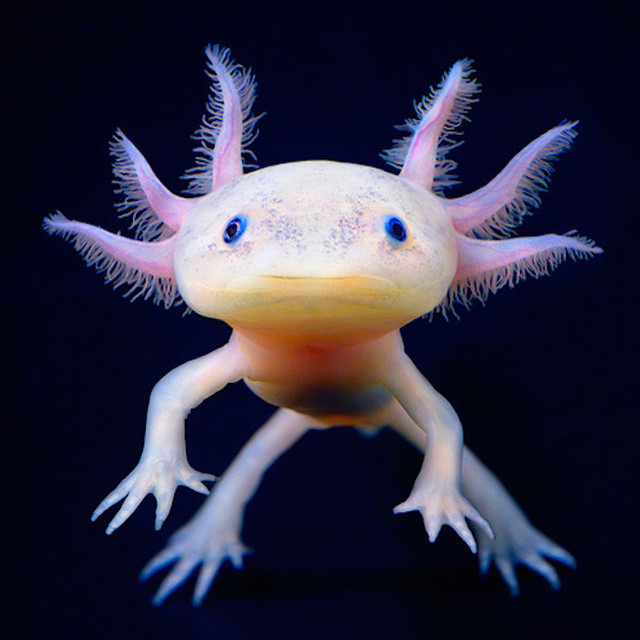
\includegraphics[width=\textwidth]{../pics/axolotl_animal-1.jpg}
\end{columns}

\medskip

\onslide<2>{
\begin{quote}
``[Axolotl] combines the .. forward secrecy [of] a hash iteration ratchet like SCIMP [with the] future secrecy .. of a DH ratchet like OtR'' % \\
\hfill --- Moxie Marlinspike % (TextSecure)
}
\end{quote}
\end{frame}


\begin{frame}{Axolotl ratchet by Trevor Perrin and Moxie Marlinspike}
\begin{columns}[T]
\column{0.6\textwidth}
Approach: \\
\hspace*{2pt} Run DH whenever possible \\
% \hspace*{5pt} 2-step vs 3-step \\
\hspace*{2pt} Iterate key by hashing otherwise 

\bigskip
2-step DH is less book keeping than OtR's 3-step DH \\

\medskip
Header is one DH public key, \\
\hspace*{2pt} which one can encrypt.

\onslide<2>{
\bigskip
Neutral against Shor's algorithm \\
 \hspace*{2pt} running on a quantum computer. \\
}

\column{0.4\textwidth}
\includegraphics[width=\textwidth]{../pics/axolotl_diagram}
% \vspace*{-20pt}
% \includegraphics[width=0.95\textwidth,trim={0 0 0 47},clip]{axolotl_diagram}
\end{columns}
\end{frame}


% Metadata : entropique2015.tex

% Tor : ...


\begin{frame}{Sphinx by George Danezis and Ian Goldberg}
\begin{center}

\includegraphics[width=0.8\textwidth]{../pics/Sphinx}
% Mixnets use cryptography in mysterious ways

An asychnornous mixnet allows us defeat corrolation attacks that best Tor
\end{center}
\end{frame}


\begin{frame}{Sphinx by George Danezis and Ian Goldberg}
Sphinx is a {\em compact} packet format for mix networks.

\bigskip

Sphinx is provably secure in the universal composability model \\
\hspace*{2pt} [Camenisch \& Lysyanskaya '05, Canetti '01]
\begin{enumerate}
\item Provides correct onion routing
\item Integrity, meaning immunity to long-path attacks
\item Security, including \\
\hspace*{2pt} wrap-resistance{\small $^*$} and \\
\hspace*{2pt} indistinguishability of forward and reply messages
\item[] Replay protection implemented by Bloom filter
\end{enumerate}

\bigskip
\bigskip

{\small $^*$ Wrap-resistance helps prevent nodes from acting as decryption oracles.}
\end{frame}


\begin{frame}{Sphinx by George Danezis and Ian Goldberg}
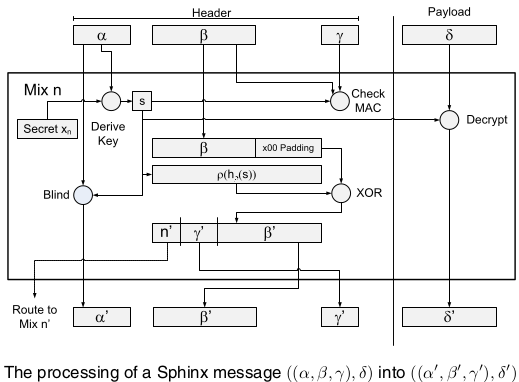
\includegraphics[width=\textwidth]{../pics/Sphinx-diagram}
\end{frame}
% LIONNESS???


% delevery : 32c3.tex


\begin{frame}{Post-quantum Sphnx?}

A quantum computer factored 15 without cheating last year. \\
That might not sound like much progress for 20 years, but \\
\hspace*{3pt}  one should expect slow progress to continue, and \\
\hspace*{3pt}  one cannot expect negative results. \\

\medskip

We could worry for many decades even if they are impossible!

\end{frame}


\begin{frame}{Post-quantum Sphnx?}

We have two seemingly post-quantum key exchanges :
\begin{itemize}
\item Ring learning with errors and
\item Super-singular isogenies Diffie Hellman 
\end{itemize}

\medskip
In both cases, we need a blinding operations persumably based on
 the key exchange operation, but..
\begin{itemize}
\item anonymity is far more delicate than cryptography,
\item blinding is more fragile than key exchange, 
\item fewer researchers will ever study blinding, ..
\end{itemize}

\smallskip

And blinding is weakened by using multiple systems!

\end{frame}


\begin{frame}[t]{Ratchet for Sphinx}
\begin{columns}[T]
\column{0.60\textwidth}

Idea : Axolotl is neutral against Shor. % quantum computers.

\medskip

Can we integrate a ratchet with Sphinx?

\medskip
Axolotl won't work because : 
\begin{itemize}
\item Relays never message users
\item Cannot reuse curve elements
\end{itemize}

\medskip
Ideas : 
\begin{itemize}
\item Relays share new keys with the whole network for replay protection \\
% \hspace*{2pt} Key lifetime = SURB lifetime
\item Users should learn what messages made it eventually
\end{itemize}

\column{0.40\textwidth}
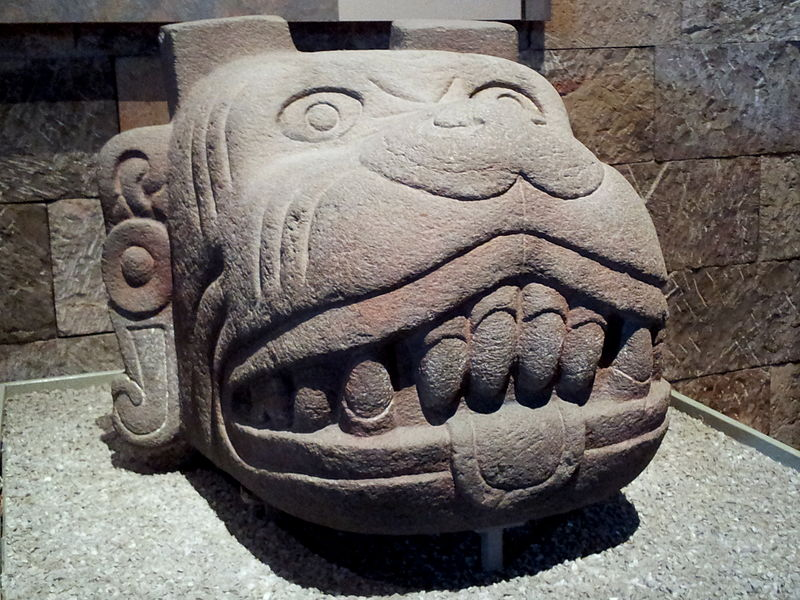
\includegraphics[width=1.35\textwidth,trim={80 0 0 0},clip]{../pics/Xolotl_muz}
\begin{center}
Xolotl \\
Sphinx + Axolotl
\end{center}
\end{columns}

\end{frame}


\begin{frame}[t]{Relay key replacement }
Replay protection requires that relays replace keys regularly. 
\begin{columns}[T]
\column{0.6\textwidth}
{\hfil Key lifetime = SURB lifetime \hfil}

\medskip
Longer lifetime improves:
\begin{itemize}
\item Delivery convenience
\end{itemize}

\smallskip
Shorter lifetime improves:
\begin{itemize}
\item Throughput 
\item Memory footprint
\item Forward-secrecy
\end{itemize}

\column{0.4\textwidth}
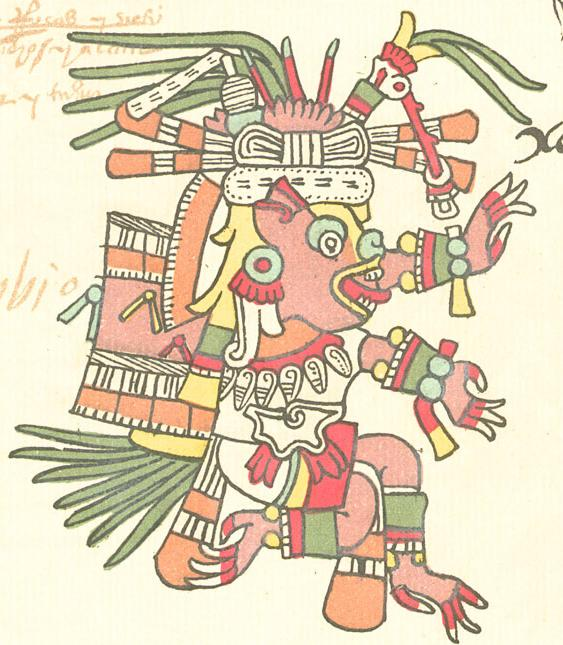
\includegraphics[width=1.2\textwidth]{../pics/Xolotl}
\end{columns}
\end{frame}


\begin{frame}[t]{Acknowledging ratchet state }
\begin{columns}[T]
\column{0.5\textwidth}
Idea: Client directs ratchet state

\bigskip
Chain keys evolve like Axolotl, 
 \hspace*{2pt} producing leaf keys. % \\ not message keys.

\smallskip
Create message keys by hashing \\
 \hspace*{2pt} a leaf key with a Sphinx ECDH \\ % result.

\smallskip
 \hspace*{10pt} $\textrm{mk} = H(\textrm{lk},H'(\textrm{ECDH}(\textrm{u},\textrm{r})))$

\medskip
\onslide<2>{
Packets identify the message key from which their chain started.

\smallskip % \hspace*{2pt}
And their leaf key sequence no. % number.
%}

\smallskip
% \onslide<3>{ % \hspace*{2pt}
And parent max sequence no.
%And their parent chain's max sequence no.
}

\column{0.5\textwidth}
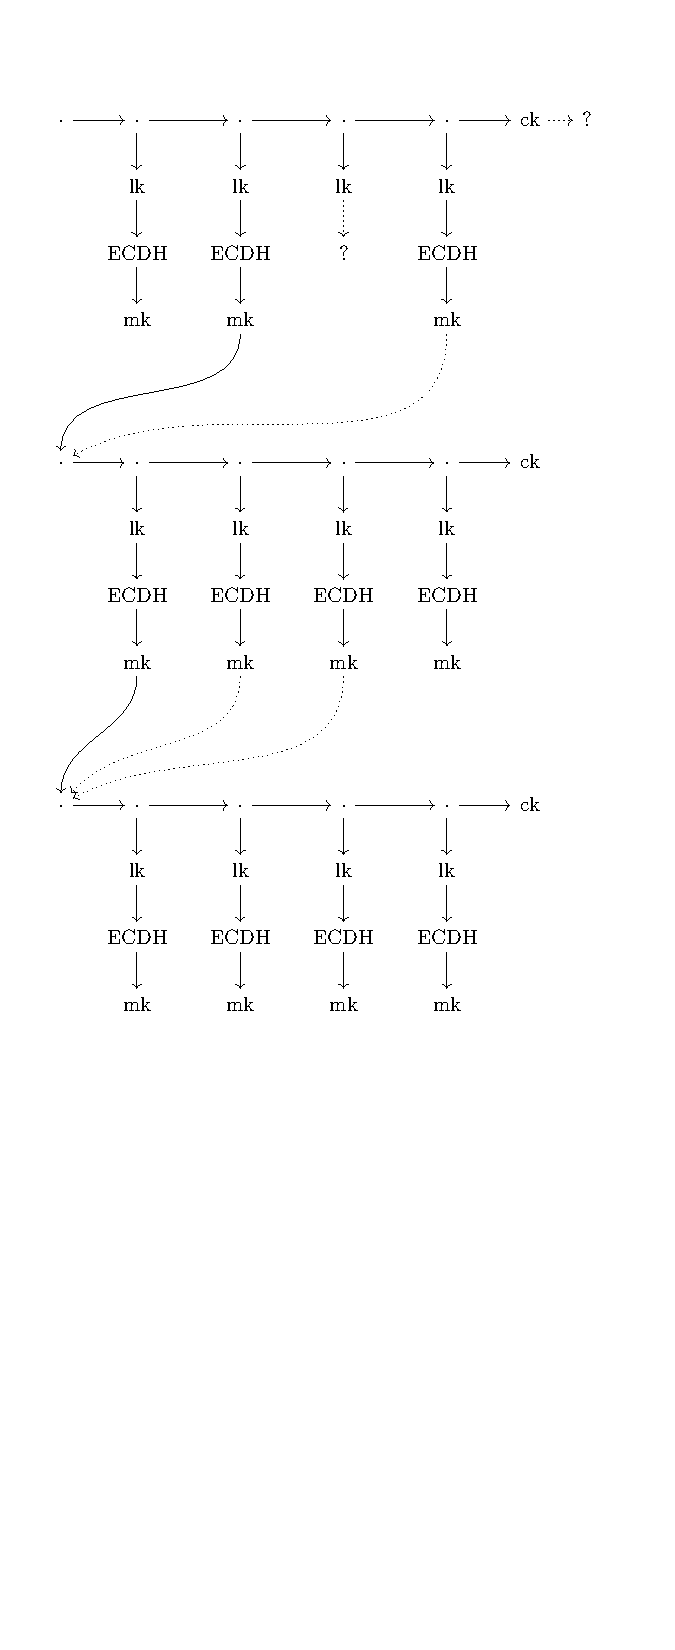
\includegraphics[width=0.95\textwidth,trim={0 0 0 47},clip]{../up/32c3/Xolotl_diagram0}
\end{columns}
\end{frame}



\begin{frame}{Wait. Aren't ratchets only pseudononymous? }

We cannot use the Xolotl ratchet for every mixnet hop, but \\
the ratchet should be suitable for certian situations.

\bigskip

Guard nodes can use a session ratchet initialized with:
\begin{itemize}
\item post-quantum key exchange, or 
\item another longer term ratchet, maybe.
\end{itemize}

\bigskip

Third hop out of a five hope circut: \\
\begin{itemize}
\item Long-term ratchet is okay, but only pseudonymous
\item Initializing from a longer term ratchet is okay
\end{itemize}

\bigskip
Other hops require greater care

\[ \textrm{User} \to \textrm{Guard} \to \textrm{Anon} \to \textrm{Pseudo} \to \textrm{Anon} \to \textrm{Cross} \to \cdots \]

\end{frame}








\end{document}









\pause\medskip
I doubted that SIDH admited the blinding used in Sphinx, \\
\hspace*{3pt} but recently my opinion has changed. \\

\smallskip

% There are nevertheless several disadvantages, like
% \begin{itemize}
% \item 0.5kb+ public keys, and
% \item 300 times slower than curve25519!
% \end{itemize}

We'd need composing isogenies to give a blinding operation too. 

\smallskip

And SIDH is 300 times slower than curve25519 anyways!










\begin{frame}{A Ring-LWE straw-man Sphinx}

We have a ring $R = (\Z/p\Z)[x]/\Phi(x)$ where ... \\
\hspace*{3pt} $\Phi(x)$ is irreducible of degree 1024, maybe cyclotomic,
 and $p>1024$ is prime. 
\smallskip

A private key is polynomials $s$ and $e$ with small coefficents, \\
\hspace*{3pt} while a public key is a random $a\in R$ and $b = s a + e$.

\pause\smallskip
A candidate blinding operation might be, pick $s'$, $e'$, and $e''$ small, \\
\hspace*{3pt} to compute $a' = s' a + e'$ and $b' = s' b + e''$.

\smallskip
Imagine a path $n_1 \to n_2 \to n_3$ where $n_2$ is honest but \\
\hspace*{3pt}  $n_1$ and $n_3$ controlled by the adversary.
\begin{align*}
a' b &= (s' a + e') (s a + e) = s' s a^2 + s' a e + e' s a + e' e \\
a b' &= (s' (s a + e) + e'')a = s' s a^2 + s' e a + e'' a \\
a' b - a b' &= e' s a + e' e - e'' a
= e' b - e'' a
= (e' s - e'') a + e' e
\end{align*}

\end{frame}





